\chapter{Design}

\section{Overall System Design}

\subsection{Short description of the main parts of the system}

\subsection{System flowcharts showing an overview of the complete system}

\section{User Interface Designs}

\section{Program Structure}

\subsection{Top-down design structure charts}

\subsection{Algorithms in pseudo-code for each data transformation process}

\subsection{Object Diagrams}

\subsection{Class Definitions}

\section{Prototyping}

\section{Definition of Data Requirements}

\subsection{Identification of all data input items}

\subsection{Identification of all data output items}

\subsection{Explanation of how data output items are generated}

\subsection{Data Dictionary}

\subsection{Identification of appropriate storage media}


\newpage

\section{Database Design}

\subsection{Normalisation}
 
\subsubsection{ER Diagrams}


\begin{figure}[H]
    \caption{ER Diagram} \label{ER_Diagram.pdf}
    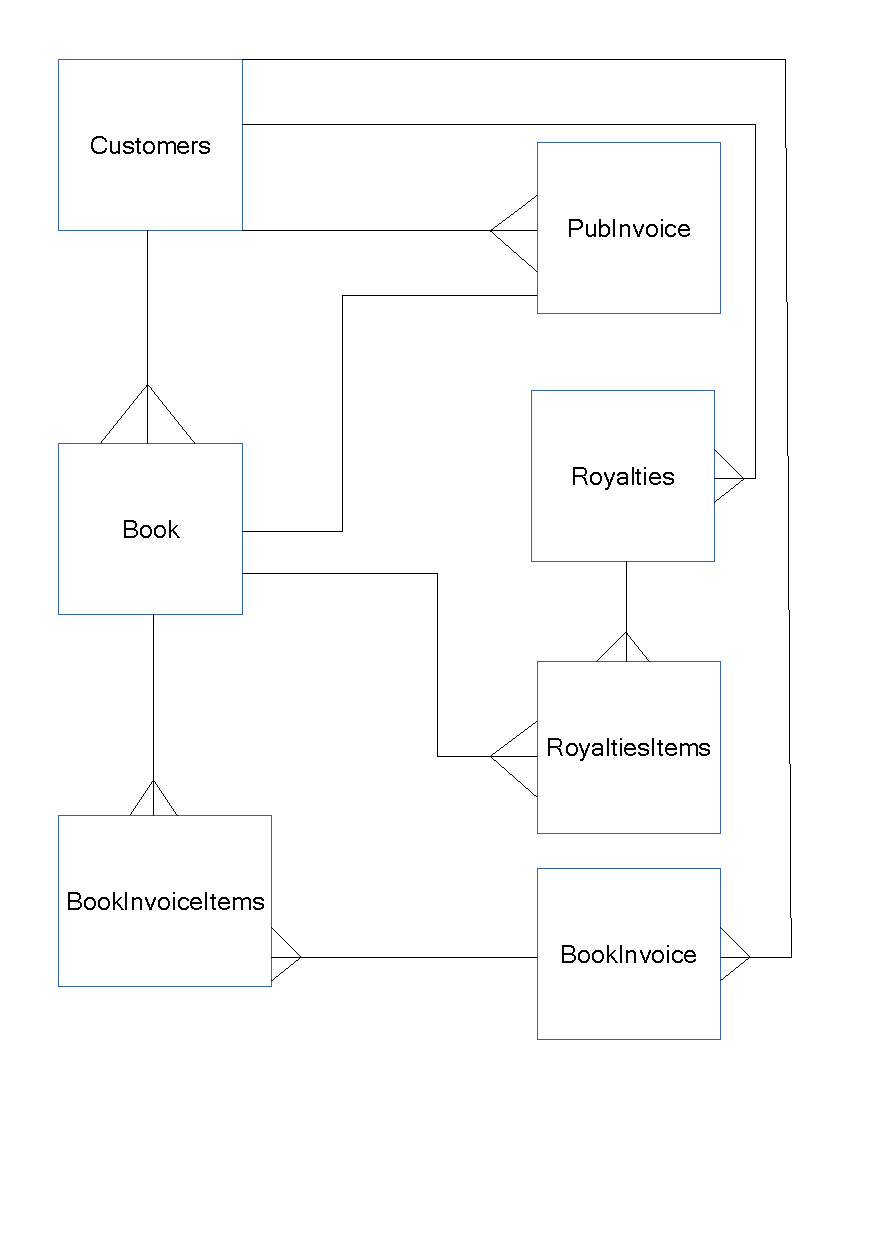
\includegraphics[width=\textwidth]{./Design/ER_Diagram.pdf}
\end{figure}


\subsubsection{Entity Descriptions}

Customer(\underline{Author ID}, FirstName, LastName, Email, Address, Postcode, Phone Number)

Invoice(\underline{InvoicePayment}, \underline{InvoiceDate}, \emph{ISBN}, \emph{AuthorID}, InvoiceQuantity, InvoiceDiscount, ShippingPrice, ShippingType)

Royalties(\underline{RoyaltyPayment}, \underline{RoyaltiesDate}, \emph{ISBN}, \emph{AuthorID}, RoyaltyDiscount, WholeSalePrice, RoyaltyQuantity, NetSales, PrintCost)

Book(\underline{ISBN}, \emph{AuthorID}, Book Title, NoOfPages, Size, Cover, Paper, Back, Paper, Font, FontSize, DatePublished, Price)

\subsubsection{UNF to 3NF}

Key:

\textbf{Bold Font} = Primary Key

\emph{Italics} = Foreign Key

Each Column represents a new group.

First of all, I have started with the data in its unnormalised form.

\begin{tabular}{|p{2.5cm}|}
    \hline
    FirstName \\
    LastName \\
    Email \\
    PhoneNumber \\
    Address \\
    PostCode \\
    AuthorID \\
    ISBN \\
    BookTitle \\
    NoOfPages \\
    Size \\
    Back \\
    Cover \\
    Paper \\
    Font \\
    FontSize \\
    DatePublished \\
    Price \\
    RoyaltyPayment \\
    RoyaltiesDate \\
    Discount \\
    WholeSalePrice \\
    Quantity \\
    NetSales \\
    PrintCost \\
    InvoicePayment \\
    InvoiceDate \\
    ShippingPrice \\
    ShippingType \\
    \hline
\end{tabular}

Then, I put it into the first normal form.

\begin{tabular}{|p{2.5cm}|p{2.5cm}|}
    \hline
    \textbf{AuthorID} & \textbf{ISBN} \\
    FirstName & \textbf{AuthorID} \\
    LastName & BookTitle \\
    Email & NoOfPages \\
    PhoneNumber & Size \\
    Address & Back \\
    PostCode & Cover \\
    & Paper \\
    & Font \\
    & FontSize \\
    & DatePublished\\
    & Price \\
    & RoyaltyPayment \\
    & RoyaltiesDate \\
    & Discount \\
    & WholeSalePrice \\
    & Quantity \\
    & NetSales \\
    & PrintCost \\
    & InvoicePayment \\
    & InvoiceDate \\
    & ShippingPrice \\
    & ShippingType \\
    \hline
\end{tabular}

After that, I put it into the second normal form.

\begin{tabular}{|p{2.5cm}|p{2.5cm}|p{2.5cm}|}
    \hline
    \textbf{AuthorID} & \textbf{ISBN} & \textbf{ISBN} \\
    FirstName & \textbf{AuthorID} & BookTitle \\
    LastName & RoyaltyPayment & NoOfPages \\
    Email  & RoyaltiesDate & Size \\
    PhoneNumber & RoyaltyDiscount & Back \\
    Address & WholeSalePrice & Cover \\
    PostCode & RoyaltyQuantity & Paper \\
    & NetSales & Font \\
    & PrintCost & FontSize \\
    & InvoicePayment & DatePublished \\
    & InvoiceDate & Price \\
    & InvoiceDiscount & \\
    & InvoiceQuantity & \\
    & ShippingPrice & \\
    & ShippingType & \\
    \hline
\end{tabular}

Finally, I put the data into its third normal form.

\begin{tabular}{|p{2.5cm}|p{2.5cm}|p{2cm}|p{3cm}|p{3cm}|}
    \hline
    \textbf{AuthorID} & \textbf{ISBN} & \textbf{ISBN} & \textbf{RoyaltyPayment} & \textbf{InvoicePayment} \\
    FirstName & \textbf{AuthorID} & \emph{AuthorID} & \textbf{RoyaltiesDate} & \textbf{InvoiceDate} \\
    LastName & \emph{RoyaltyPayment} & BookTitle & \emph{ISBN} & \emph{ISBN} \\
    Email  & \emph{RoyaltiesDate} & NoOfPages & \emph{AuthorID} & \emph{AuthorID} \\
    PhoneNumber & \emph{InvoicePayment} & Size & RoyaltyDiscount & InvoiceQuantity \\
    Address & \emph{InvoiceDate} & Back & WholeSalePrice & InvoiceDiscount \\
    PostCode & & Cover & RoyaltyQuantity & ShippingPrice \\
    & & Paper & NetSales & ShippingType \\
    & & Font & PrintCost & \\
    & & FontSize & &\\
    & & DatePublished & & \\
    & & Price & & \\
    \hline
\end{tabular}

\subsection{SQL Queries}

I am using Python to format the SQL query text strings.

\begin{tabular}{|p{10cm}|p{5cm}|}
    \hline
    \textbf{SQL} & \textbf{Descriptions} \\ \hline
     """insert into \\ Customer(FirstName, LastName, Email, PhoneNumber, Address, Postcode) values (\{0\}, \{1\}, \{2\}, \{3\}, \{4\}, \{5\}) \\ """.format(FirstName, LastName, Email, PhoneNumber, Address, Postcode) & An example of an SQL statement which adds customer records to the database. Here, it is entering a new customer record with the attributes: FirstName, LastName, Email, PhoneNumber, Address and Postcode. \\ \hline
    """create table Royalties(\\ RoyaltyPayment REAL,\\ RoyaltiesDate DATE,\\ ISBN STRING,\\ AuthorID INTEGER,\\ RoyaltyDiscount STRING,\\ WholeSalePrice REAL,\\ RoyaltyQuantity INTEGER,\\ NetSales REAL,\\ PrintCost REAL\\ PRIMARY KEY(RoyaltyPayment, RoyaltiesDate) \\ FOREIGN KEY(ISBN, AuthorID) REFERENCES \\ Book(ISBN), Customer(AuthorID) """ & An example of an SQL statement that creates a new table for the Royalties. There is a composite primary key consisting of RoyaltyPayment and RoyaltiesDate, and there are two foreign keys, which are ISBN and AuthorID. \\ \hline
\end{tabular}

\section{Security and Integrity of the System and Data}

\subsection{Security and Integrity of Data}

\subsection{System Security}

\section{Validation}

\section{Testing}

\begin{landscape}
\subsection{Outline Plan}

\begin{center}
    \begin{tabular}{|p{2cm}|p{5cm}|p{5cm}|p{4cm}|}
        \hline
        \textbf{Test Series} & \textbf{Purpose of Test Series} & \textbf{Testing Strategy} & \textbf{Strategy Rationale}\\ \hline
        Example & Example & Example & Example \\ \hline
    \end{tabular}
\end{center}

\subsection{Detailed Plan}

\begin{center}
    \begin{longtable}{|p{1.5cm}|p{2.5cm}|p{2.5cm}|p{2cm}|p{2cm}|p{2cm}|p{2cm}|p{2cm}|}
        \hline
        \textbf{Test Series} & \textbf{Purpose of Test} & \textbf{Test Description} & \textbf{Test Data} & \textbf{Test Data Type (Normal/ Erroneous/ Boundary)} & \textbf{Expected Result} & \textbf{Actual Result} & \textbf{Evidence}\\ \hline
        Example & Example & Example & Example & Example & Example & Example & Example \\ \hline
    \end{longtable}
\end{center}
\end{landscape}